\documentclass{article}

\usepackage{geometry}
\geometry{left=3cm,right=3cm,top=2cm,bottom=2cm}
\usepackage[utf8]{inputenc}
\usepackage{amsmath, amsfonts, amssymb, amsthm}
% \usepackage[framemethod=default]{mdframed}% was framemethod=TikZ
\usepackage{mathrsfs}
\usepackage{comment}
\usepackage{enumerate}
\usepackage{xcolor}
\usepackage{titlesec}
\usepackage{setspace}
\usepackage{hyperref}
\hypersetup{
colorlinks=true,
allcolors=orange
}
\usepackage{cleveref}

\usepackage[most]{tcolorbox}
\usepackage{ragged2e}
\usepackage{todonotes}
\usepackage{cleveref}
\usepackage{mathtools}
\usepackage{svg, float}

% \usepackage[sectionbib]{natbib}
% \usepackage{chapterbib}


\definecolor{astral}        {RGB}{46,116,181}
\definecolor{cb-blue}       {RGB}{70, 130, 180}
\definecolor{orange}        {RGB}{214,150, 92}


% Name of the author!!!
\newcommand{\aut}{AUTHOR}

%
\titleformat*{\section}{\LARGE \bfseries}
\titleformat*{\subsection}{\Large \bfseries}
\titleformat*{\subsubsection}{\Large \bfseries}
% \titleformat*{\paragraph}{\large \bfseries}
\titleformat*{\subparagraph}{\large \bfseries}


%%%%%%%%%%%%%%%%%%%%%%%%%%%%%%%%%%%%%%%%%%%%%%%%%%%%%%%%%%%%
% General 
\newcommand{\nextline}{\hfill\break}
\newcommand{\nl}{\nextline\rm}

\DeclareMathOperator*{\esssup}{ess\,sup}

\newcommand{\defeq}{\stackrel{\text{def.}}{=}}
% FA and LA
% inner product: \inne{a}{b}
\newcommand{\inne}[2]{\left<{#1},{#2}\right>}

% norm: \norm{a}
\newcommand{\norm}[1]{\left\|{#1}\right\|}

% Curly H
\newcommand{\hbs}{$\mathscr{H}$ }
\newcommand{\hbp}{\mathscr{H}}

% Dual : \dual{x}
\newcommand{\dual}[1]{{#1}^*}

% Sequence from 1  to infty: \sequ{x_n}
\newcommand{\sequ}[1]{\left({#1}\right)_1^\infty}

% f: A-> B \func{f}{A}{B}
\newcommand{\func}[3]{${#1}:{#2}\xrightarrow{}{#3}$}

% interior
\newcommand{\interior}{\textrm{int}}

% Bounded linear funcs
\newcommand{\blf}[2]{\mathcal{L}({#1},{#2})}

\newcommand{\prf}{\textit{proof}:   }



% Fields 
\newcommand{\real}{\mathbb{R}}
\newcommand{\qq}{\mathbb{Q}}
\newcommand{\comp}{\mathbb{C}}
\newcommand{\inte}{\mathbb{Z}}
\newcommand{\natu}{\mathbb{N}}
%%%%%%%%%%%%%%%%%%%%%%%%%%%%%%%%%%%%%%%%%%%%%%%%%%%%%%%%%%%%



% If theoremstyle is n
    % Theorems
    % \newtheorem{example}{Example}[subsection]
    % \newtheorem{definition}[example]{Definition}
    % \newtheorem{proposition}[example]{Proposition}
    % \newtheorem{remark}[example]{Remark}
    % \newtheorem{theorem}[example]{Theorem}
    % \newtheorem{lemma}[example]{Lemma}
    % \newtheorem{corollary}[example]{Corollary}


% for numbering the theorems            
% \theoremstyle{plain}
% %%%%%%%%%%%%%%%%%%%%%%%%%%%%%%%%%%%%%%%%%%%%%%%%%%%%%%%%%%%
% \newtheorem{theorem}{Theorem}[section]
% \newtheorem{lemma}[theorem]{Lemma}
% \newtheorem{corollary}[theorem]{Corollary}
% \newtheorem{proposition}[theorem]{Proposition}
% %%%%%%%%%%%%%%%%%%%%%%%%%%%%%%%%%%%%%%%%%%%%%%%%%%%%%%%%%%%
% % the following are not in italics
% \theoremstyle{definition}
% \newtheorem{definition}[theorem]{Definition}
% \newtheorem{example}[theorem]{Example}
% \newtheorem{remark}[theorem]{Remark}
% \newtheorem{claim}[theorem]{Claim}
%%%%%%%%%%%%%%%%%%%%%%%%%%%%%%%%%%%%%%%%%%%%%%%%%%%%%%%%%%%%

% proof box
\newtcbtheorem[no counter]{pf}{Proof}{
  enhanced,
  rounded corners,
  attach boxed title to top,
  colback=white,
  colframe=black!25,
  fonttitle=\bfseries,
  coltitle=black,
  boxed title style={
    rounded corners,
    size=small,
    colback=black!25,
    colframe=black!25,
  } 
}{prf}


% clever ref settings
\crefname{lemma}{lemma}{lemmas}
\Crefname{lemma}{Lemma}{Lemmas}
\crefname{theorem}{theorem}{theorems}
\Crefname{theorem}{Theorem}{Theorems}
%%%%%%%%%%%%%%%%%%%%%%%%%%%%%%%%%%%%%%%%%%%%%%%%%%%%%%%%%%%%
% formatting 
% https://tex.stackexchange.com/questions/217497/aligning-stackrel-signs-beneath-each-other-using-split
\newlength{\leftstackrelawd}
\newlength{\leftstackrelbwd}
\def\leftstackrel#1#2{\settowidth{\leftstackrelawd}%
{${{}^{#1}}$}\settowidth{\leftstackrelbwd}{$#2$}%
\addtolength{\leftstackrelawd}{-\leftstackrelbwd}%
\leavevmode\ifthenelse{\lengthtest{\leftstackrelawd>0pt}}%
{\kern-.5\leftstackrelawd}{}\mathrel{\mathop{#2}\limits^{#1}}}
%%%%%%%%%%%%%%%%%%%%%%%%%%%%%%%%%%%%%%%%%%%%%%%%%%%%%%%%%%%%

%%%%%%%%%%%%%%%%%%%%%%%%%%%%%%%%%%%%%%%%%%%%%%%%%%%%%%%%%%%%
% colors
\usepackage{xcolor}
\definecolor{royal}{RGB}{0,35,102}
\definecolor{navyblue}{cmyk}{1,0.5,0,0.3}
\definecolor{c0}{cmyk}{0.83, 0.34, 0, 0.29}
\definecolor{c1}{cmyk}{0, 0.5, 0.95, 0}
\definecolor{c2}{cmyk}{0.72, 0, 0.72, 0.37}
\definecolor{skyblue}{cmyk}{0.6,0.16,0,0}
\definecolor{lightgreen}{cmyk}{0.5,0,0.5,0}
\definecolor{pastelgreen}{cmyk}{0.25,0,0.25,0}
\definecolor{mossgreen}{cmyk}{0.64,0.4,1,0}
\definecolor{reddish}{cmyk}{0, 0.64, 0.64, 0.2}
\definecolor{one}{cmyk}{0, 0.6, 0.46, 0.69}
\definecolor{two}{cmyk}{0.11, 0, 0.72, 0.16}
\definecolor{imperialorange}{RGB}{255,134,24}
%%%%%%%%%%%%%%%%%%%%%%%%%%%%%%%%%%%%%%%%%%%%%%%%%%%%%%%%%%%%
% spacing
% \onehalfspacing
\RaggedRight
%%%%%%%%%%%%%%%%%%%%%%%%%%%%%%%%%%%%%%%%%%%%%%%%%%%%%%%%%%%%


% modify innerrightmargin if floats were lost

\usepackage{amsfonts, amsmath, amssymb, amsthm, thmtools, bm}
\usepackage{avant} % Use the Avantgarde font for headings
\usepackage[most]{tcolorbox}

% Boxed/framed environments
\newtheoremstyle{royalnumbox}%
{0pt}% Space above
{0pt}% Space below
{\normalfont}% Body font
{}% Indent amount
{\small\bf\color{royal}}% Theorem head font
{\;}% Punctuation after theorem head
{0.25em}% Space after theorem head
{ \color{royal} 
    \thmname{#1} 
    \thmnumber{#2} \thmnote{\bfseries\color{black}---\nobreakspace#3.}} % Optional theorem note
\renewcommand{\qedsymbol}{$\blacksquare$}% Optional qed square

\newtheoremstyle{blacknumex}% Theorem style name
{5pt}% Space above
{5pt}% Space below
{\normalfont}% Body font
{} % Indent amount
{\small\bf}% Theorem head font
{\;}% Punctuation after theorem head
{0.25em}% Space after theorem head
{
    \thmname{#1}
    \thmnumber{#2}
    \thmnote{---\nobreakspace#3.}}% Optional theorem note

\newtheorem*{notation}{Notation}
\newtheorem*{hint}{Hint}
\newtheorem*{solution}{Solution}

\newcounter{dummy} 
\numberwithin{dummy}{section}

\theoremstyle{royalnumbox}
\newtheorem{definitionT}[dummy]{Definition}
\newtheorem{theoremT}[dummy]{Theorem}
\newtheorem{lemmaT}[dummy]{Lemma}
\newtheorem{corollaryT}[dummy]{Corollary}
\newtheorem{propositionT}[dummy]{Proposition}
\newtheorem{propertyT}[dummy]{Property}
\newtheorem{remarkT}[dummy]{Remark}

\theoremstyle{blacknumex}
\newtheorem{exampleT}[dummy]{Example}
\newtheorem{exerciseT}[dummy]{Exercise}

\numberwithin{equation}{section}

\RequirePackage[framemethod=TikZ]{mdframed}

\newcounter{definition}

% % Definition box
% \newtcolorbox{dBox}{
%   enhanced,
%   breakable,
%   arc=5pt, outer arc=5pt,
%   colback=reddish!10, 
%   colframe=reddish,
%   boxrule=1pt,
%   left=5pt, 
%   right=5pt, 
%   top=5pt, 
%   bottom=5pt,
% %   skipabove=7pt, skipbelow=7pt
% }



% % Main Theorem box
% \newtcolorbox{tBox}{
%   enhanced,
%   breakable,
%   arc=5pt, 
%   outer arc=5pt,
%   colback=c0!10, 
%   colframe=c0!10,
%   boxrule=1pt,
%   left=5pt, 
%   right=5pt, 
%   top=5pt, 
%   bottom=5pt,
% %   skipabove=7pt, skipbelow=7pt
% }


% % Lemma/Corollary/Proposition/Property box
% \newtcolorbox{lBox}{
%   enhanced,
%   breakable,
%   arc=5pt,
%   outer arc=5pt,
%   colback=c0!10,
%   colframe=c0!10,
%   boxrule=1pt,
%   left=5pt,
%   right=5pt,
%   top=5pt,
%   bottom=5pt,
% %   skipabove=7pt, skipbelow=7pt
% }

% % Example/Remark/Exercise box
% \newtcolorbox{exBox}{
%   enhanced,
%   breakable,
%   arc=5pt, 
%   outer arc=5pt,
%   colback=mossgreen!10!white,
%   colframe=mossgreen,
%   boxrule=1pt,
%   left=5pt,
%   right=5pt,
%   top=5pt,
%   bottom=5pt,
% %   skipabove=7pt, skipbelow=7pt
% }

% % Extra content box for contents not covered in the lecture notes
% \newtcolorbox{unexamBox}{
%   enhanced,
%   breakable,
%   arc=20pt, 
%   outer arc=20pt,
%   colback=gray!10,
%   colframe=gray,
%   boxrule=1pt,
%   left=5pt, 
%   right=5pt, 
%   top=5pt, 
%   bottom=5pt,
% %   skipabove=7pt, skipbelow=7pt
% }

% Definition box
\newtcolorbox{dBox}{
  enhanced,
  breakable,
  arc=5pt, outer arc=5pt,
  colback=skyblue!10,  % Light blue
  colframe=skyblue,    % Blue
  boxrule=1pt,
  left=5pt, 
  right=5pt, 
  top=5pt, 
  bottom=5pt,
}

% Main Theorem box
\newtcolorbox{tBox}{
  enhanced,
  breakable,
  arc=5pt, 
  outer arc=5pt,
  colback=yellow!10,   % Light yellow
  colframe=yellow!80!black, % Dark yellow
  boxrule=1pt,
  left=5pt, 
  right=5pt, 
  top=5pt, 
  bottom=5pt,
}

% Lemma/Corollary/Proposition/Property box
\newtcolorbox{lBox}{
  enhanced,
  breakable,
  arc=5pt,
  outer arc=5pt,
  colback=orange!10,   % Light orange
  colframe=orange!80!black, % Dark orange
  boxrule=1pt,
  left=5pt,
  right=5pt,
  top=5pt,
  bottom=5pt,
}

% Example/Remark/Exercise box
\newtcolorbox{exBox}{
  enhanced,
  breakable,
  arc=5pt, 
  outer arc=5pt,
  colback=teal!10!white,   % Light teal
  colframe=teal,           % Teal
  boxrule=1pt,
  left=5pt,
  right=5pt,
  top=5pt,
  bottom=5pt,
}

% Extra content box for contents not covered in the lecture notes
\newtcolorbox{unexamBox}{
  enhanced,
  breakable,
  arc=20pt, 
  outer arc=20pt,
  colback=gray!10,    % Light gray
  colframe=gray,      % Gray
  boxrule=1pt,
  left=5pt, 
  right=5pt, 
  top=5pt, 
  bottom=5pt,
}

\newenvironment{unexaminable}{\begin{unexamBox}}{\end{unexamBox}}




% Creates an environment for each type of theorem and assigns it a theorem text style from the "Theorem Styles" section above and a colored box from above
\newenvironment{definition}{\begin{dBox}\begin{definitionT}}{\end{definitionT}\end{dBox}}

\newenvironment{theorem}{\begin{tBox}\begin{theoremT}}{\end{theoremT}\end{tBox}}

\newenvironment{lemma}{\begin{lBox}\begin{lemmaT}}{\end{lemmaT}\end{lBox}}

\newenvironment{proposition}{\begin{lBox}\begin{propositionT}}{\end{propositionT}\end{lBox}}

\newenvironment{corollary}{\begin{lBox}\begin{corollaryT}}{\end{corollaryT}\end{lBox}}

\newenvironment{property}{\begin{lBox}\begin{propertyT}}{\end{propertyT}\end{lBox}}


\newenvironment{remark}{\begin{exBox}\begin{remarkT}}{\end{remarkT}\end{exBox}}

\newenvironment{example}{\begin{exBox}\begin{exampleT}}{{}\end{exampleT}\end{exBox}}
\usepackage{tikz}
\usepackage[colon, sort&compress]{natbib}
\title{Preliminaries}

\date{\today}

\begin{document}
% \author{\aut}
\maketitle

\section{Preliminaries}
In this course, we use the terms network and graph interchangeably. A graph/network is a pair $G=(V, E)$, where $E \subseteq V \times V$. An edge is thus a pair $(u,v) \in E$. 

\begin{figure}[H]
    \centering
    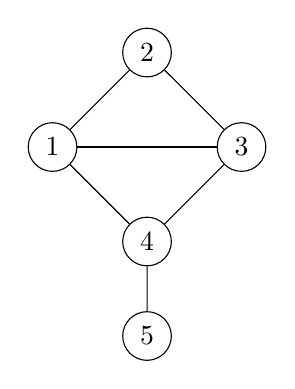
\begin{tikzpicture}[scale=1.2, every node/.style={circle, draw, minimum size=0.5cm}]
  \node (A) at (0,0) {1};
  \node (B) at (2,0) {3};
  \node (C) at (1,1) {2};
  \node (D) at (1,-1) {4};
  \node (E) at (1,-2) {5};
  
  % \draw (A) -- (B) node[midway, below] {Edge 1};
  % \draw (B) -- (C) node[midway, right] {Edge 2};
  % \draw (A) -- (C) node[midway, above, sloped] {Edge 3};
  \draw (A) -- (B) ;
  \draw (B) -- (C) ;
  \draw (A) -- (C) ;
  \draw (B) -- (D) ;
  \draw (A) -- (D) ;
  \draw (E) -- (D) ;
\end{tikzpicture}
    \caption{A graph with $|V|=5$}
    \label{fig: example graph}
\end{figure}

\begin{definition}
    A \textbf{path} in a graph is an alternating sequence of vertices and edges given by 
    \[
    \mathcal{P} = (v_0, e_1, v_1, e_2, \ldots, e_n,v_n)
    \]
    If there is a path between every pair of vertices, the graph is called \textbf{connected}.   
\end{definition}  

The length of a path is the \textbf{number of edges} in the path.

\subsection{Representations} 

In this course, we use the adjacency matrix to represent graphs. The following definiton (taken from the lectures) is for a simple graph, where there is at most one edge between any pair of vertices.  

\begin{definition}
    The \textbf{adjacency matrix} of a graph $G=(V,E)$ is a $n\times n$ matrix $A$ with each entry $(A)_{uv}$ for each pair of vertices $(u,v)\in E$ defined as:
    \begin{singlespace}
        \begin{equation*}
         (A)_{uv} = \begin{cases}
            1 & \mathrm{if} \ u\sim v \\
            0 & \mathrm{otherwise}
        \end{cases}
    \end{equation*}
    \end{singlespace}
    where we denote $n=|V|$.
\end{definition}  

In the example above, the adjacency matrix is given by:

\begin{equation*}
        A=\begin{pmatrix}
         0&  1&  1&  1& 0\\
         1&  0&  1&  0& 0\\
         1&  1&  0&  1& 0\\
         1&  0&  1&  0& 1\\
         0&  0&  0&  1& 0\\
    \end{pmatrix}
    % \caption{Adjacency matrix for $\mathcal{G}$}
    \label{tab:adj}
\end{equation*}


Some commonly discussed (deterministic) graphs include
\begin{itemize}
    \item \textbf{The complete graph} has $\binom{n}{2}$ edges, with an adjacency matrix with all entries being $1$ except for the diagonal entries. 
    \item \textbf{The} $k$\textbf{-partite graph} see \citep{DiestelReinhard2017GT}
    \item \textbf{The star graph} is a $K_{1,k}$ partite graph, with $v_1$ being the central vertex and $v_2, \ldots, v_{k-1}$ being the vertices attached to it. The 2-star is a triangle missing an edge. 
\end{itemize}


\begin{figure}[H]
    \centering
    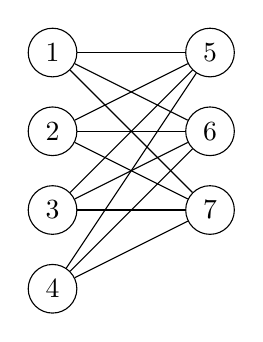
\begin{tikzpicture}
% Define the left set of vertices
\foreach \x in {1,2,3,4}
    \node[draw, circle] (\x) at (0, -\x) {\x};
% Define the right set of vertices
\foreach \y in {5,6,7}
    \node[draw, circle] (\y) at (2, -\y+4) {\y};
% Add edges between the sets
\foreach \x in {1,2,3,4}
    \foreach \y in {5,6,7}
        \draw (\x) -- (\y);
\end{tikzpicture}
    \caption{A bipartite graph $K_{4,3}$}
    \label{fig: example bipartite}
\end{figure}


They admit adjacency matrices with special structures.

\subsection{Summary Statistics}
When dealing with large graphs, it would be convenient to have simple statistics that reveal information about the underlying structure.  

\begin{itemize}
    \item  The \textbf{density} of a network is given by $\frac{2e}{n(n-1)}$
    \item The \textbf{average degree} of a network is given by $\bar{d}=\frac{1}{n}\sum_{v\in V} \sum_{u\in V, u\neq v} a_{uv}$, where $a_{uv}$ is the entry in the adjacency matrix
    \item The \textbf{degree sequence} of a given network on $V$ is the set of degrees $\{d(v): v\in V\}$
    \item The \textbf{degree distribution} is a vector with each element $d_k=\frac{1}{n} |D_k|$, where $D_k$ is the set of vertices with degree $k$
\end{itemize}
\begin{remark}
    In Sheet 1, we will see that given a sequence of non-negative integers, there is an algorithm (\textbf{Havel-Hakimi}) to determine if this sequence is a degree sequence. (if so we call it graphical)
\end{remark}

\begin{definition}
    The \textbf{global clustering coefficient} (often abbreviated as just the clustering coefficient) is defined as
    \begin{equation*}
        C = \frac{\sum_{u,v,w \in V} a_{uv}a_{vw}a_{wu}}{\sum_{v \in V} d(v)(d(v)-1)}
    \end{equation*}
    where the numerator is $6\times$the number of triangles and the denominator is the number of paths of length $2$:
    \[
        C = \frac{6\times \text{number of triangles}}{\text{number of 2-paths}}
    \]
    Also, note that the number $6$ arises from the fact that we have $3!=6$ ways to choose an ordered triplet.
\end{definition}

 Note that if we divide both by $2$, then the denominator is the number of $2-$stars in the graph.

A similar statistic is the local clustering coefficient for a particular vertex $v$.

\begin{definition}
    The \textbf{local clustering coefficient} of $v$ is given by:
    \begin{equation*}
        C(v) =  \frac{\sum_{u,w \in V} a_{uv}a_{vw}a_{wu}}{d(v)(d(v)-1)} 
        % = \frac{\frac{1}{2}\sum_{u,w \in N(v), u\neq w} a_{uv}a_{wv}}{\binom{d(v)}{2}}
    \end{equation*}
    where the numerator is $2\times$the number of triangles and the denominator is the number of paths of length $2$ containing $v$:
    \[
        C(v) = \frac{2\times \text{number of triangles containing } v}{\text{number of 2-paths containing }v}
    \]
\end{definition}
Note the denominator has an alternative form $\sum_{u, w \in N(v), u\neq w} a_{uv}a_{wv}$, where $N(v)$ denotes the neighbourhood of $v$; to see this, note we first sum over all pairs $(u,w)$ and then subtract the cases where they are equal, which gives $d(v)^2-d(v)$, as desired.

Thus, the \textbf{average local clustering coefficient} is 
\[
    \overline{C}=\frac{1}{|V|}\sum_{v \in V} C(v)
\]

Aside from statistics that arise from degrees of vertices, the global structure is also captured by paths in graphs. 

\begin{definition}
    The \textbf{average shortest path} is given by:
    \[
        \ell = \frac{1}{|V|(|V|-1)} \sum_{u\neq v, u,v\in V} \ell (u,v)
    \]
    where $\ell(u,v)$ is the length of the shortest path between $u$ and $v$.
\end{definition}

\begin{remark}
    We can compute $\ell(u,v)$ from the smallest power of adjacency matrix $A$ such that the $(u,v)^{th}$ entry of $A^p$ is non-zero. (This can be shown by induction)
\end{remark}

\begin{definition}
    The \textbf{motif} of a graph is a small, over-represented subgraph, where over-representation is judged using a probabilistic model for the network.
\end{definition}

\newpage
\bibliographystyle{apalike}
\bibliography{bibliography1.bib}

\end{document}